% https://tex.stackexchange.com/a/159294/316176
\newcommand{\rulesep}{\unskip\ \vrule\ }

\begin{figure*}
  \centering
  \begin{subfigure}[b]{0.33\textwidth}
    \centering
    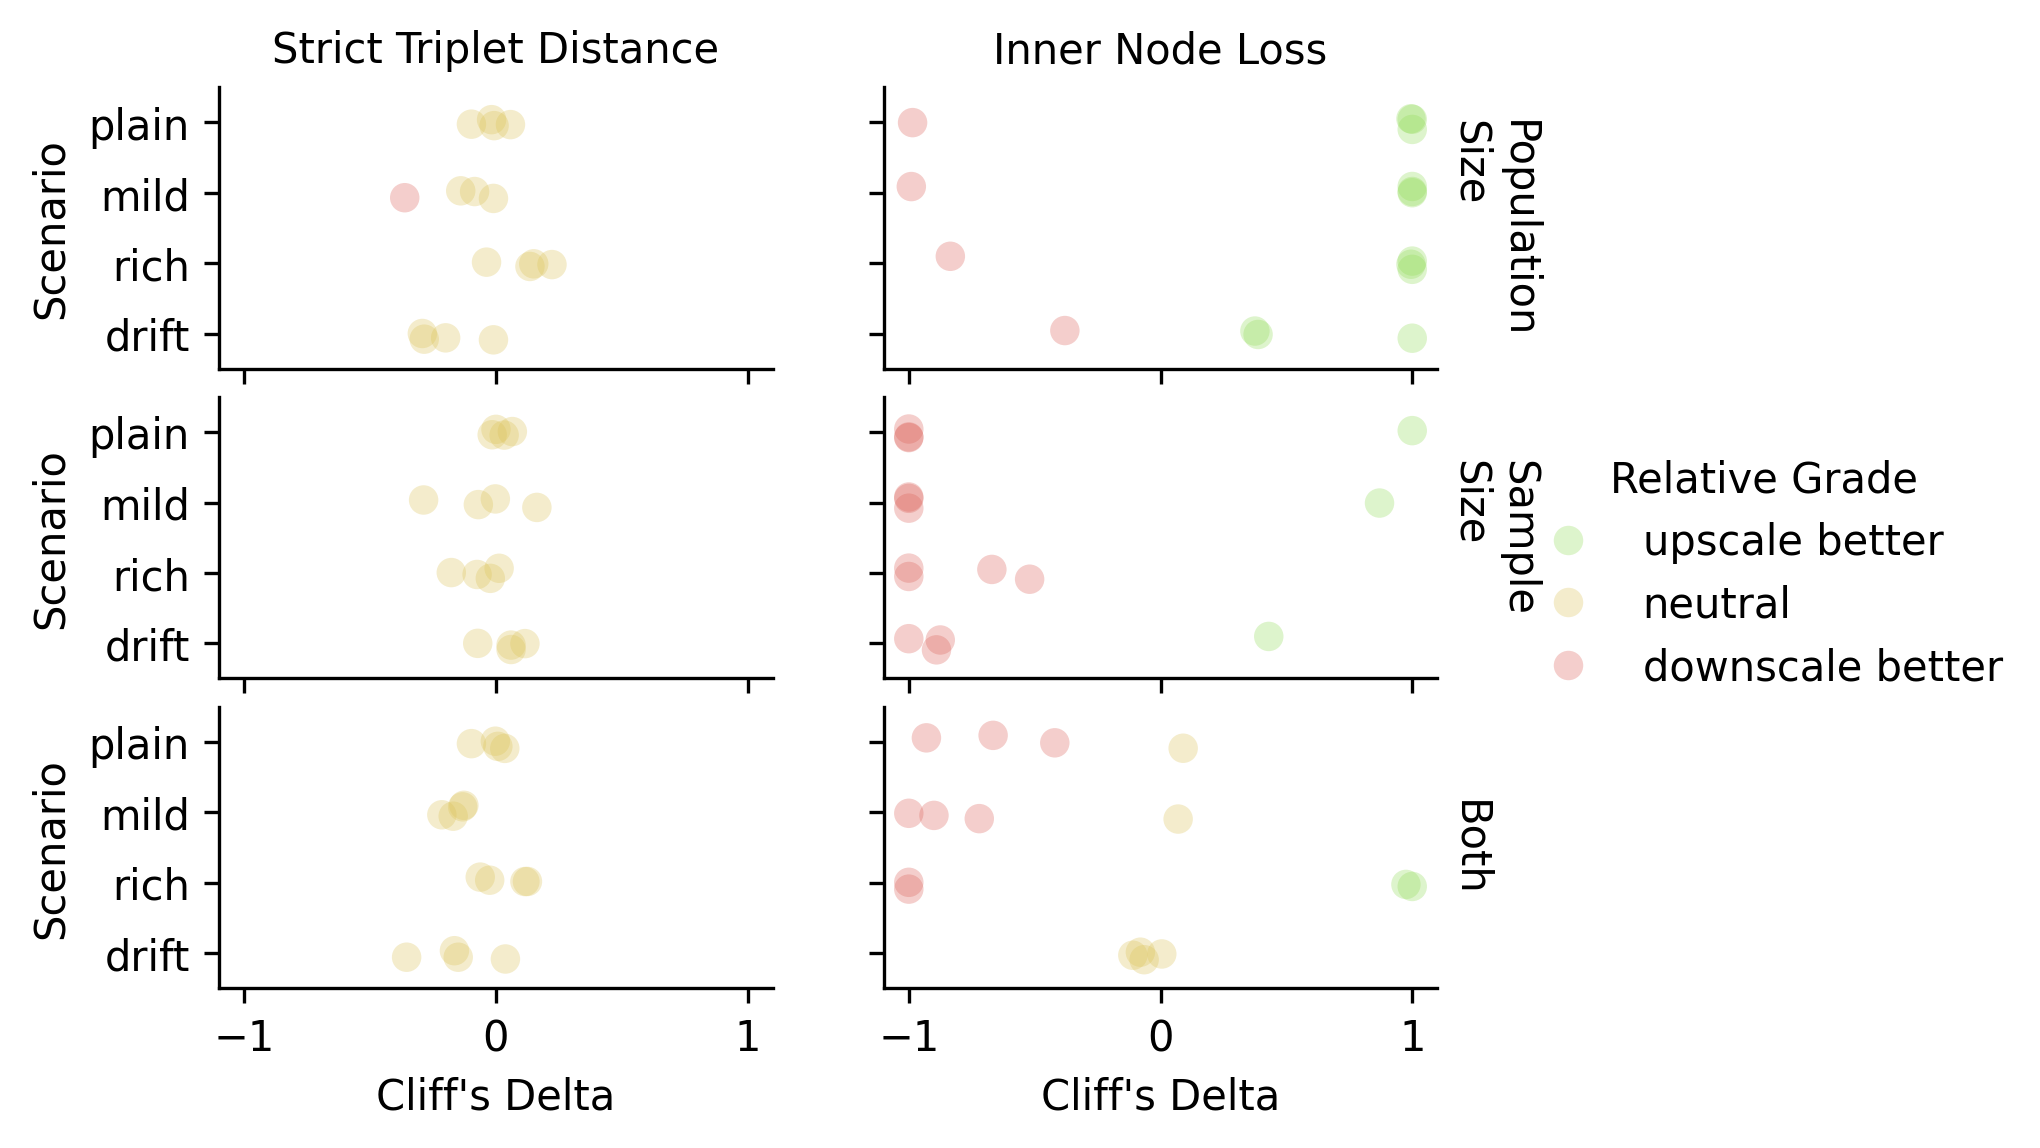
\includegraphics[height=1.7in,trim={0 0 5cm 0},clip]{binder/binder/dsamp-popsize-scale/teeplots/col=metric+hue=relative-grade+kind=strip+policy=tilted+row=scaling-factor+viz=catplot+x=cliff-s-delta+y=scenario+ext=}
    \caption{tilted}
  \end{subfigure}%
  \rulesep %
  \begin{subfigure}[b]{0.26\textwidth}
    \centering
    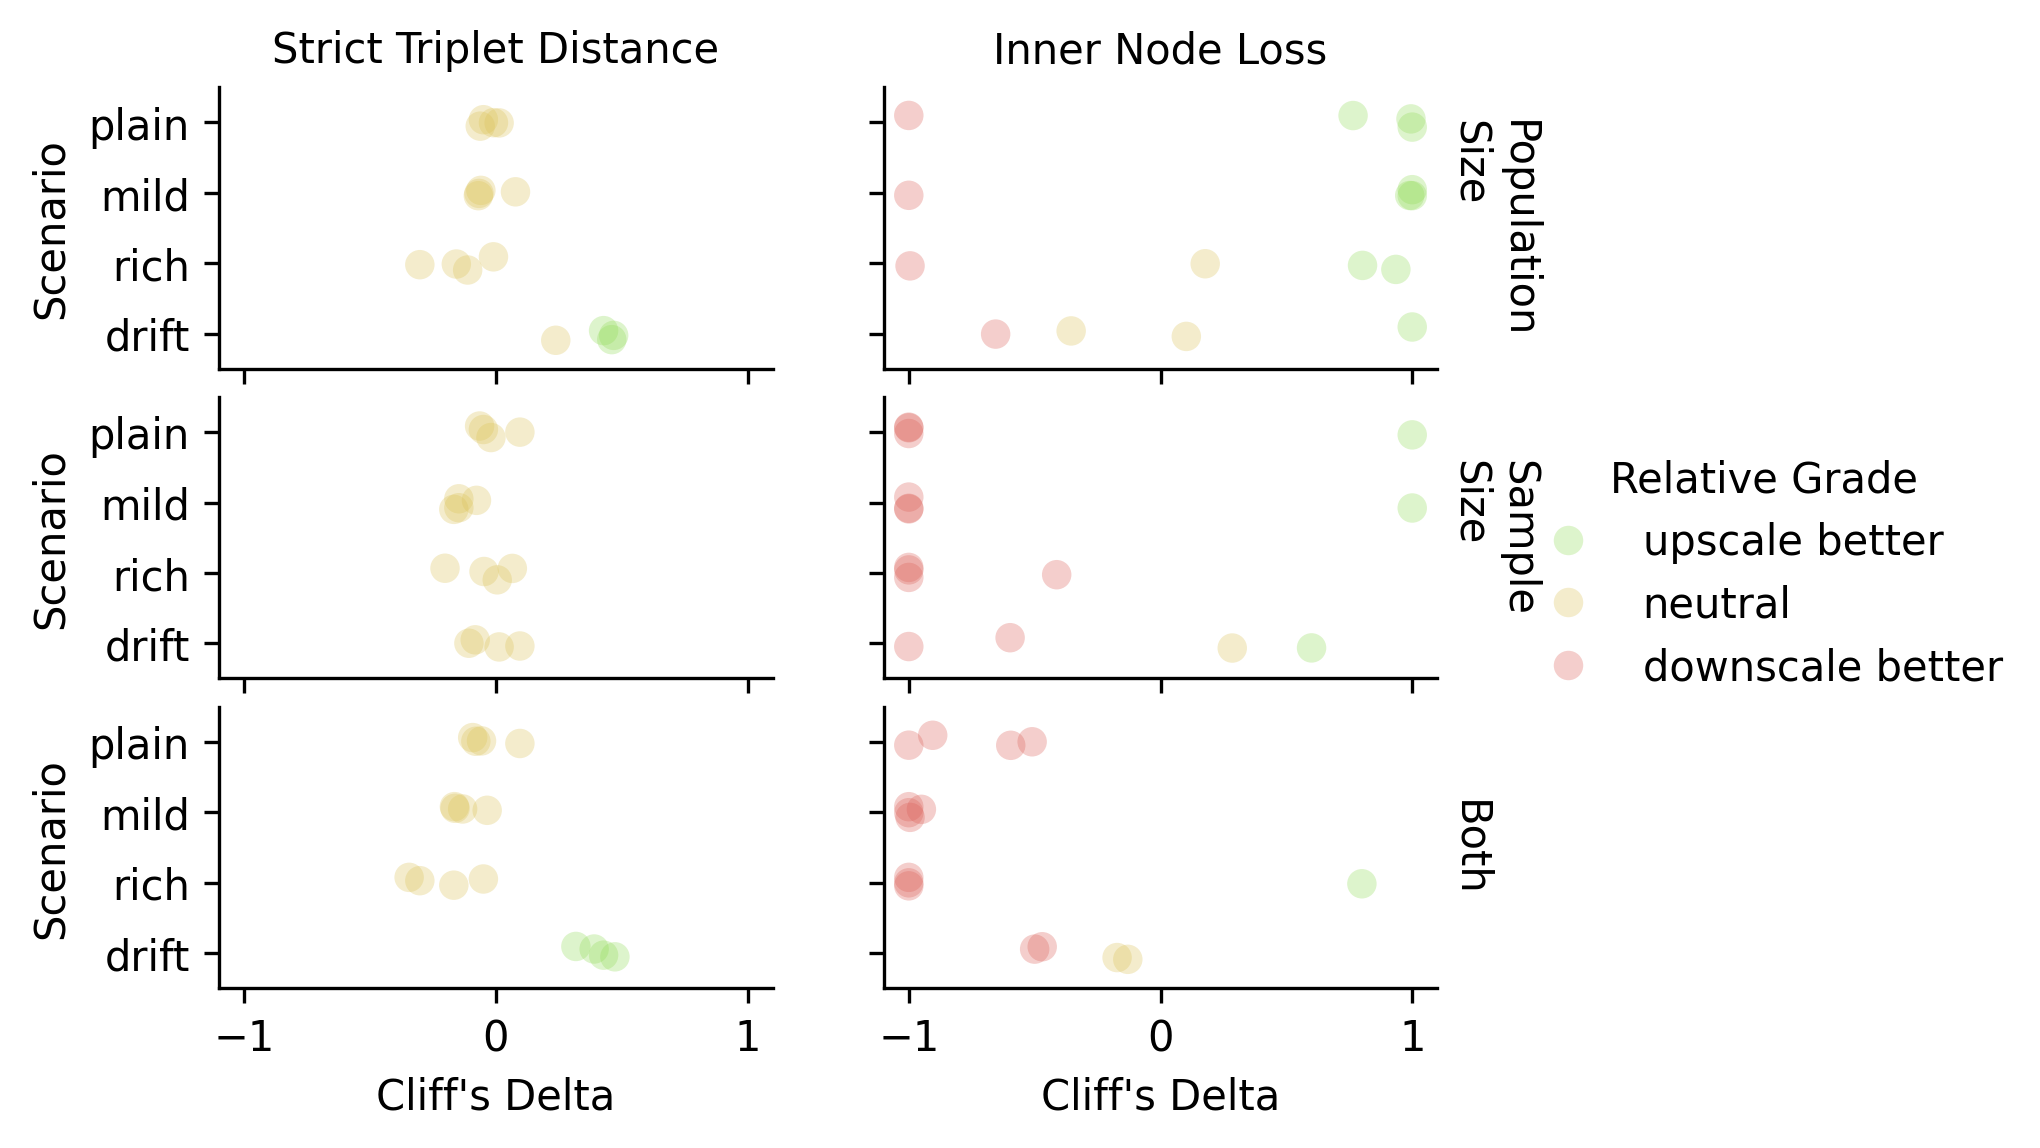
\includegraphics[height=1.7in,trim={2cm 0 5cm 0},clip]{binder/binder/dsamp-popsize-scale/teeplots/col=metric+hue=relative-grade+kind=strip+policy=hybrid+row=scaling-factor+viz=catplot+x=cliff-s-delta+y=scenario+ext=}
    \caption{hybrid}
  \end{subfigure}%
  \rulesep %
  \begin{subfigure}[b]{0.39\textwidth}
    \centering
    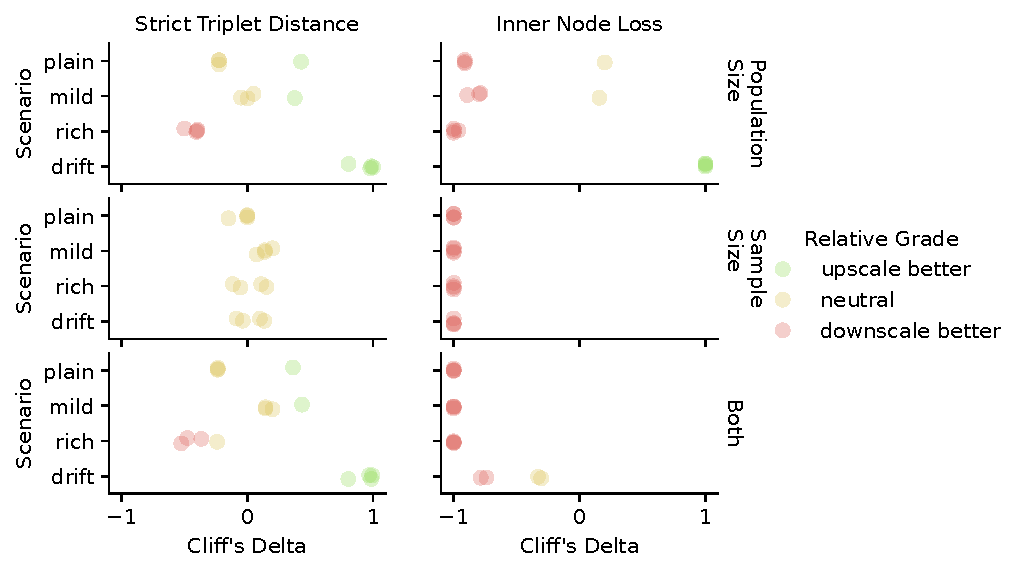
\includegraphics[height=1.7in,trim={2cm 0 0 0},clip]{binder/binder/dsamp-popsize-scale/teeplots/col=metric+hue=relative-grade+kind=strip+policy=steady+row=scaling-factor+viz=catplot+x=cliff-s-delta+y=scenario+ext=}
    \caption{steady}
  \end{subfigure}
  \caption{Population size and sample size scaling relationships.}
  \label{fig:scaling-summary}
\end{figure*}